\h{Theoretical Framework}
\section{Core Mechanisms}

\begin{refsection}[references/0001_2_theoretical.bib]

Energetically Coherent Computation (ECC) proposes that consciousness emerges from specific patterns of energy organization within biological neural systems. Unlike traditional computational approaches that view consciousness as abstract information processing \cite{dehaene2014toward}, ECC grounds conscious experience in the physical dynamics of energy flows, coherence, and thermodynamic constraints within the brain.

Central to ECC is the concept that consciousness requires more than mere energy dissipation or information processing—it demands specific forms of energetic coherence that allow for stable yet adaptive conscious states. These coherent states emerge from the interplay of several key mechanisms: continuous energy flows organized through transcriptomic profiles that create region-specific alphabets for encoding conscious states, dynamic feedback loops that maintain stability while allowing for adaptation, and thermodynamic constraints that ensure efficient, low-entropy processing within the neural architecture \cite{varela2001brainweb}.

The framework differs fundamentally from traditional computational models by emphasizing that consciousness cannot be reduced to abstract symbolic manipulation or discrete state transitions. Instead, ECC suggests that conscious experience requires continuous, physically embodied energy dynamics that achieve coherence across multiple scales—from molecular interactions to global brain states \cite{buzsaki2006rhythms}. This coherence is maintained through what ECC terms the "neural light cone," which defines the spatial and temporal boundaries within which conscious states can maintain causal connectivity and energetic stability.

These core mechanisms work together to create a rich alphabet of conscious states—a diverse yet structured set of possible configurations that allow for complex representation while maintaining energetic efficiency. This alphabet is not arbitrary but is shaped by the specific transcriptomic profiles of different brain regions, allowing for specialized processing while maintaining global coherence through mechanisms of mutual feedback and dynamic stability \cite{hasson2015hierarchical}.

The interplay between these mechanisms gives rise to energetically coherent fields—stable configurations of energy that can sustain conscious experience while remaining adaptable to changing conditions. At the cellular level, neurons and astrocytes form complex networks where energy flows are regulated through gap junctions and synaptic connections \cite{vasile2017human}. However, unlike traditional neural network models that focus solely on information transmission, ECC emphasizes how these cellular networks achieve coherent energy states through continuous feedback between electrical, chemical, and metabolic processes.

Rather than viewing thermal fluctuations as mere noise to be overcome, ECC suggests that the brain leverages these fluctuations to achieve dynamic stability, allowing consciousness to remain coherent while adapting to changing conditions \cite{singer2018neuronal}. This stands in contrast to digital computational systems, which must actively suppress noise to maintain discrete state transitions. The framework emphasizes the importance of interface dynamics—the ways in which different brain subsystems interact and maintain coherence across boundaries \cite{sporns2011networks}.

This organization allows conscious states to achieve faithful representation—the capacity to reflect both internal and external conditions while maintaining coherence and enabling adaptive responses. Unlike simpler dissipative structures, conscious systems can sustain complex patterns of energy flow that encode rich, context-sensitive information while maintaining thermodynamic efficiency \cite{fries2015rhythms}.

The culmination of these mechanisms—energetic coherence, thermal noise regulation, and interface dynamics—enables the brain to achieve a form of unified conscious experience while respecting physical and thermodynamic constraints. This unity, however, is not absolute or all-encompassing. Rather, ECC suggests that consciousness emerges as a selective, bounded phenomenon where only regions capable of maintaining appropriate energetic coherence participate in conscious experience at any given moment \cite{tononi2015consciousness2dup}.

A critical insight of the framework is that these mechanisms operate within specific spatial and temporal boundaries determined by what ECC terms the "neural light cone." This concept, borrowed from relativistic physics but adapted to neural dynamics, describes the limits within which conscious integration can occur. Just as nothing can travel faster than light in physics, there are fundamental limits to how quickly and how far conscious integration can propagate through the brain's networks while maintaining coherence \cite{von2010dynamic}.

These boundaries help explain several persistent questions in consciousness research, including why not all brain regions participate in consciousness simultaneously and why certain cognitive processes remain unconscious. The neural light cone provides a physical basis for these limitations, showing how they emerge naturally from the constraints on energy propagation and coherence maintenance within biological neural systems \cite{atasoy2016human}.

The framework draws particular attention to the role of electromagnetic fields in consciousness, suggesting they provide an essential substrate for information integration and coherent processing \cite{mcfadden2020integrating, pockett2012electromagnetic}. These fields operate in concert with other mechanisms, including neural oscillations and phase synchronization, to maintain the coherent states necessary for conscious experience \cite{brunel2003what}.

Recent theoretical work has suggested that quantum effects may play a role in these coherent processes, though the exact nature of this contribution remains a matter of ongoing investigation \cite{hameroff2014consciousness2dup}. While ECC does not depend on quantum mechanisms for its core principles, it remains open to their potential role in fine-tuning or modulating coherent states.

Understanding these core mechanisms provides a foundation for investigating how conscious experience emerges from physical systems while remaining grounded in established principles of neuroscience and physics. This theoretical framework suggests new approaches to studying consciousness, emphasizing the need to consider energy dynamics and coherence patterns alongside traditional measures of neural activity.

\section{Neural Light Cones}

The concept of neural light cones provides a powerful framework for understanding how conscious experience maintains coherence while remaining bounded by physical constraints. Drawing inspiration from relativistic physics, where light cones define the possible causal relationships between events in spacetime, neural light cones describe the regions of the brain that can maintain causal connectivity and energetic coherence within the temporal windows required for conscious processing \cite{herzog2016time}.

Just as a light cone in physics determines which events can causally influence each other given the speed of light, a neural light cone defines the spatial and temporal boundaries within which brain regions can achieve the coherent energy dynamics necessary for conscious experience \cite{northoff2017how}. This bounded region is determined by several factors: the propagation speed of neural signals, the maintenance of energetic coherence, and the thermodynamic constraints on information integration \cite{bekenstein1981universal}.

Within a neural light cone, energy flows must maintain sufficient coherence to support conscious processing. This requires a delicate balance between stability and adaptability, achieved through the continuous interaction of multiple mechanisms. Neurons and astrocytes within the cone maintain synchronized activity patterns, while gap junctions and synaptic connections enable rapid signal propagation that preserves informational and energetic coherence \cite{melloni2007synchronization}. The boundaries of the neural light cone are not fixed but dynamic, shifting based on metabolic conditions, attention, and task demands.

Critically, the neural light cone concept helps explain why consciousness cannot extend arbitrarily across space and time. Just as physical causality is limited by the speed of light, conscious integration is limited by the speed of neural signal propagation and the maintenance of energetic coherence \cite{delcul2007brain}. This explains why, for instance, widely separated brain regions cannot achieve direct conscious integration without intermediate processing steps, and why consciousness requires a minimum temporal window for integration.

The neural light cone framework also provides insight into the structure of conscious experience. Regions within the cone can maintain the coherent energy dynamics necessary for conscious processing, while areas outside the cone may support cognitive function without directly contributing to conscious experience \cite{zylberberg2010brain}. This selective inclusion in consciousness is not arbitrary but follows directly from the physical constraints on maintaining energetic coherence across neural networks.

\begin{figure}[h]
    \centering
    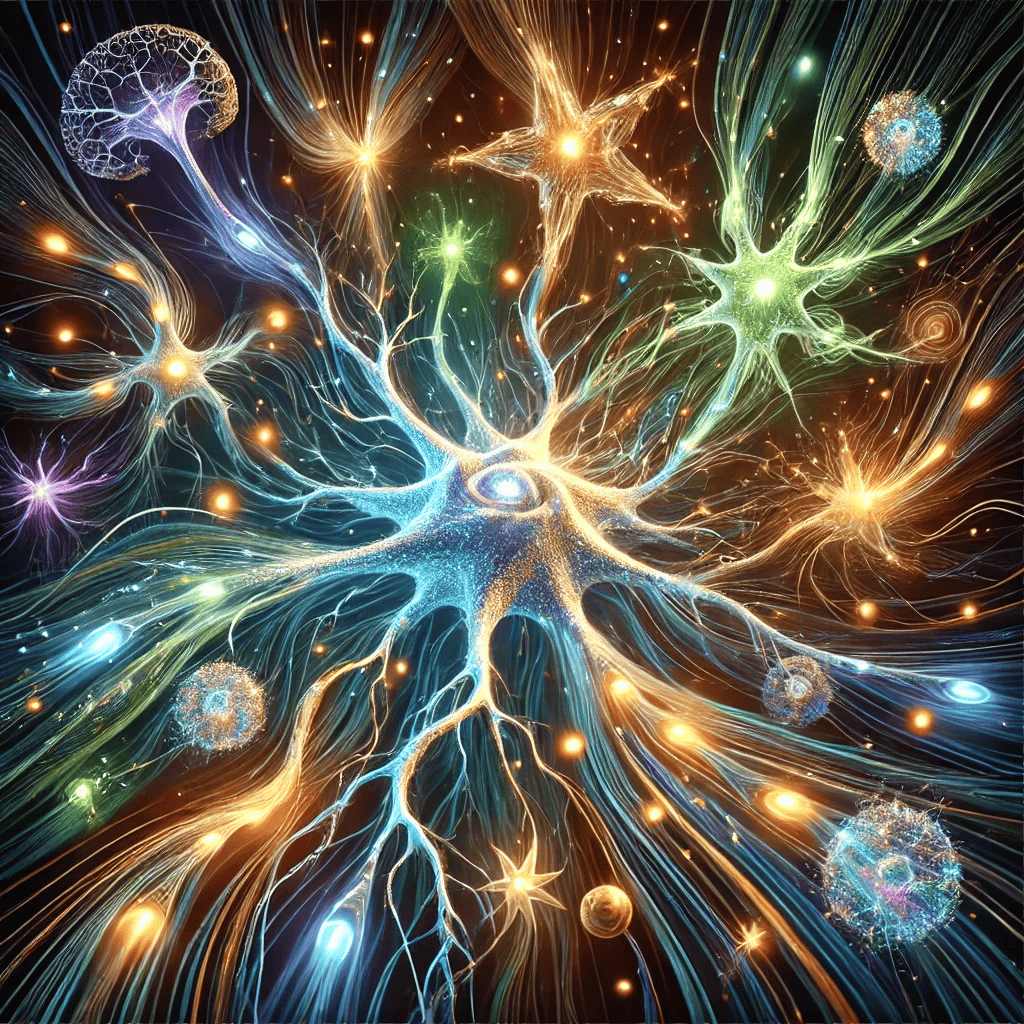
\includegraphics[width=0.8\textwidth]{light_cones.png}

    \caption{Neural light cones as a shorthand for boundary conditions of consciousness}
\end{figure}

The neural light cone concept extends beyond simple spatial and temporal boundaries to encompass the organization of energetic coherence itself. Within each cone, multiple scales of organization—from molecular interactions to regional activation patterns—must maintain alignment to support conscious processing \cite{vazquez2019gradients}. This multi-scale coherence is achieved through triangulation, where different regions within the cone maintain stable relationships through continuous mutual feedback and adjustment.

A key feature of neural light cones is their role in maintaining synchronic and diachronic unity—the integration of conscious experience across space and time respectively. Synchronic unity emerges from the capacity of regions within the cone to achieve simultaneous coherence, while diachronic unity depends on the stable propagation of coherent states across successive temporal windows \cite{tegmark2016improved}. This dual unity is maintained through the continuous operation of feedback loops that stabilize energy flows while allowing for adaptive changes in response to new inputs.

The boundaries of neural light cones are partially determined by thermal noise thresholds, which act as natural limits on the maintenance of coherent energy states \cite{oyama2009noise}. Regions within the cone must maintain sufficient energetic coherence to overcome these thermal fluctuations, while areas that cannot sustain such coherence effectively fall outside the conscious field. This creates a natural selection mechanism for conscious participation, where only those regions capable of maintaining appropriate energetic stability contribute to conscious experience.

Importantly, neural light cones are not isolated structures but form overlapping fields of influence across the cortical sheet. This overlap allows for smooth transitions in conscious experience, as different regions enter and exit the conscious field based on attention, task demands, and metabolic conditions \cite{petermann2009spontaneous}. The interaction between overlapping light cones basically creates a global light cone—a broader field of conscious integration that nonetheless remains bounded by the physical constraints on neural coherence.

The implications of the neural light cone framework extend beyond explaining current conscious experience to inform our understanding of fundamental limitations in consciousness. For instance, the model provides clear reasons why consciousness cannot be "uploaded" or transmitted across arbitrary distances—such processes would necessarily break the continuous, causally-connected energy flows that the light cone maintains \cite{seth2015granger}. Similarly, it explains why consciousness differs fundamentally from sleep states, where energy coherence patterns are altered but not destroyed, versus death, where the capacity for coherent energy maintenance is irreversibly lost.

The neural light cone also helps resolve long-standing questions about the relationship between conscious and unconscious processing. Rather than positing a rigid boundary between conscious and unconscious states, the model suggests a dynamic interface where regions move in and out of conscious awareness based on their ability to maintain coherent energy states within the light cone's boundaries \cite{tononi1998consciousness}. This fluid boundary allows for the brain's remarkable ability to shift attention and integrate new information while maintaining a stable conscious field.

Perhaps most significantly, the neural light cone framework bridges local and global aspects of conscious experience. By describing how local coherence patterns can align and integrate within broader fields of conscious awareness, it provides a physical basis for both the unity and diversity of conscious experience \cite{ramachandran2001synaesthesia}. This integration occurs through mechanisms of mutual recursion and continuous feedback, allowing for coherent diversity—the capacity to maintain distinct local patterns while contributing to a unified global experience.

The implications extend to understanding phenomena such as synaesthesia and other altered states of consciousness, where unusual patterns of integration within the neural light cone may lead to non-typical conscious experiences \cite{abraham1996metaplasticity}. The framework suggests that such phenomena emerge from modifications to the normal boundaries and integration patterns of neural light cones, rather than from purely computational or representational changes.

Understanding how neural light cones enable both local processing and global integration leads naturally to consideration of the temporal dimensions of consciousness—specifically, how the brain maintains both moment-to-moment awareness (synchronic unity) and continuous experience across time (diachronic unity) \cite{hoel2017when}. This theoretical foundation provides a bridge between the physical mechanisms of neural processing and the phenomenological features of conscious experience, suggesting new approaches to investigating both normal and altered states of consciousness.

\section{Synchronic and Diachronic Unity}

The unity of conscious experience represents one of the most compelling yet challenging aspects of consciousness to explain mechanistically. ECC approaches this challenge by distinguishing between two fundamental forms of unity—synchronic and diachronic—while showing how both emerge from underlying principles of energetic coherence within the brain's neural architecture \cite{engel2001temporal}.

Synchronic unity refers to the moment-to-moment integration of diverse conscious contents into a single, unified field of experience. Within ECC's framework, this unity is achieved not through a central processor or global workspace, but through the aligned dynamics of multiple brain regions maintaining coherent energy states \cite{singer1999neuronal}. This alignment occurs through mutual recursion, where regions continuously update their states in response to each other while maintaining stable energy patterns. Crucially, this synchronic unity operates within the constraints of the neural light cone, meaning that only regions capable of maintaining appropriate energetic coherence can participate in the unified conscious field at any given moment \cite{gray1999temporal}.

Diachronic unity describes the continuous thread of consciousness that persists across time, creating our sense of an unbroken stream of experience. ECC proposes that this temporal continuity emerges from the brain's ability to maintain stable energy configurations while smoothly transitioning between states \cite{honey2012slow}. This process relies on what might be called coherence inheritance, where each moment's conscious state builds upon and incorporates aspects of previous states while integrating new information.

The interaction between these two forms of unity is mediated by several key mechanisms. First, the brain's astrocytic networks provide a slower, more stable background against which faster neural dynamics can play out, helping to maintain continuity across moments while allowing for rapid updates to conscious content. Second, the rich alphabet of possible conscious states—defined by region-specific transcriptomic profiles—enables smooth transitions between different conscious configurations while maintaining overall coherence \cite{womelsdorf2007modulation}.

This fundamental distinction between synchronic and diachronic unity helps resolve longstanding questions about how consciousness maintains both its moment-to-moment integration and its temporal continuity \cite{vanrullen2003perception}. Understanding how these different aspects of unity emerge from patterns of energetic coherence provides new insight into both the stability and flexibility of conscious experience, while suggesting specific mechanisms through which this unity might be disrupted in various pathological conditions \cite{fell2011role}.

The maintenance of both forms of unity depends critically on coherence gradients across the cortical sheet. These gradients represent structured transitions in energy states that allow different brain regions to maintain local specificity while participating in global integration \cite{adhikari2010cross}. Unlike simpler models that posit binary transitions between conscious and unconscious processing, ECC suggests that consciousness involves continuous gradients of coherence that enable smooth transitions both spatially (across regions) and temporally (between moments).

A key insight of ECC is that synchronic and diachronic unity are not simply parallel processes but are fundamentally interlinked through shared mechanisms of energy organization \cite{wang2010neurophysiological}. The same principles that enable moment-to-moment integration of conscious contents also facilitate the smooth transition between conscious states over time. This dual role is particularly evident in the brain's handling of temporal boundaries within consciousness—the way it bridges the gap between discrete neural events and our experience of continuous, flowing consciousness \cite{vanrullen2003perception}.

However, ECC suggests that the apparent global unity of consciousness may itself be partially illusory—what we might call the framerate illusion \cite{panzeri2010sensory, harris2019conscious}. While local regions maintain genuine coherence through direct energetic coupling, the sense of complete global unity likely represents a useful fiction generated by our cognitive architecture. Much as film creates the illusion of continuous motion through discrete frames, consciousness may achieve its apparent seamlessness through sophisticated management of coherent states rather than genuine moment-to-moment continuity across the entire brain \cite{crick1990towards}.

This perspective on the partial illusoriness of global unity leads naturally to consideration of the classical binding problem \cite{roskies1999binding}. How does the brain combine different features and qualities into coherent percepts while maintaining both differentiation and integration? The binding problem represents one of the most persistent challenges in cognitive neuroscience \cite{treisman1996binding}, and ECC offers novel insights through its framework of energetic coherence and neural light cones.

\subsection{The (neural) binding problem}

The neural binding problem—how the brain integrates distributed information into unified conscious experiences—takes on new significance within Energetically Coherent Computation (ECC). While traditional accounts focus on synchronized neural firing or information integration, ECC reframes binding through the lens of energetic coherence and continuous dynamics across the cortical sheet \cite{hardcastle1999binding}.

In ECC, binding emerges from the physical organization of energy flows rather than computational synchronization alone. The framework suggests that consciousness achieves both synchronic unity (coherent experience at a moment) and diachronic unity (continuity across time) through stable, low-entropy energy fields that span relevant brain regions. These fields allow distributed information to cohere naturally through their physical dynamics, rather than requiring an explicit binding mechanism \cite{vondermalsburg1999binding}.

The key insight ECC offers regarding binding is that conscious unity does not require all information to be bound simultaneously across the entire brain. Instead, binding occurs within the constraints of the neural light cone—the region of causal connectivity that can influence conscious experience at a given moment. Information becomes bound when it achieves sufficient energetic coherence within this light cone, allowing it to contribute to the unified conscious field \cite{singer1999neuronal}.

This binding process is supported by several mechanisms in ECC. First, the rich alphabet encoded by region-specific transcriptomic profiles allows different areas to maintain distinct but compatible energy states \cite{kumar2010spiking}. Second, continuous triangulation between regions enables smooth integration of information across space and time. Third, mutual recursion and nested feedback loops help stabilize bound states while allowing for dynamic updating as new information arrives \cite{buzsaki2004neuronal}.

The brain's astrocytic networks play a crucial role in this binding process by providing a substrate for coherent energy distribution. Unlike neurons, which operate through discrete action potentials, astrocytes form syncytia—networks of cells connected by gap junctions that allow for continuous energy flows and ion redistribution. These networks help maintain the stable, low-entropy conditions necessary for conscious binding while also supporting the dynamic flexibility required for changing conscious states \cite{womelsdorf2007modulation}.

ECC thus suggests that the binding problem may be partially dissolved by recognizing consciousness as an emergent property of coherent energy fields rather than a computational challenge of synchronizing discrete signals. The framework implies that binding is not achieved through a central mechanism but arises naturally from the brain's capacity to maintain energetically coherent states across spatially distributed regions \cite{lisman2013theta}.

This perspective aligns with empirical observations about the limitations of conscious binding. Not all information can be bound simultaneously, and binding breaks down under certain conditions—precisely what we would expect if binding depends on maintaining coherent energy states within physical and thermodynamic constraints \cite{zeki1999toward}. ECC therefore offers a physically grounded account of how the brain achieves the remarkable feat of creating unified conscious experiences from distributed neural activity.

Building on this foundation, ECC's approach to the binding problem also illuminates why certain features of conscious experience emerge as they do. For instance, the limited bandwidth of consciousness—our inability to simultaneously bind unlimited information into awareness—follows naturally from the thermodynamic constraints on maintaining coherent energy fields \cite{gray1999temporal}. The brain can only sustain low-entropy coherence across a finite region at any moment, creating an inherent bottleneck in conscious processing.

The framework also explains the hierarchical nature of binding, where some features bind more readily than others. Primary sensory qualities like color and motion may bind easily because they achieve coherence within localized regions that have evolved specifically to maintain stable energy states for these features. More complex bindings, such as cross-modal associations or abstract concepts, require coherence across distributed networks and thus face greater thermodynamic challenges \cite{engel2001temporal}.

ECC's treatment of binding through energetic coherence also addresses the temporal aspects of conscious unity. The diachronic unity of consciousness—our sense of a continuous stream of experience—emerges from the brain's ability to maintain stable energy gradients across time while continuously updating their content \cite{fell2011role}. This creates a form of temporal binding that naturally bridges discrete neural events into smooth conscious transitions, explaining why we experience continuous change rather than discrete state shifts.

A particularly powerful aspect of ECC's approach is its ability to explain binding failures and alterations of consciousness. When energetic coherence is disrupted—whether through pathology, drugs, or extreme conditions—we see corresponding disruptions in conscious binding \cite{wang2010neurophysiological}. This ranges from subtle binding errors in everyday experience to profound dissociations in clinical conditions, all of which can be understood as disruptions to the brain's capacity to maintain coherent energy fields.

This reconceptualization of binding through ECC offers a bridge between phenomenology and physics, suggesting that the unity of consciousness is neither purely subjective nor simply computational, but emerges from fundamental physical principles operating under specific biological constraints. This provides a framework for understanding conscious unity that is both scientifically tractable and philosophically illuminating \cite{roskies1999binding}.

The binding problem, viewed through ECC's lens, thus becomes less about synchronizing discrete information and more about maintaining appropriate conditions for coherent energy fields. This shift in perspective suggests new directions for research, focusing on how biological systems achieve and maintain the specific forms of energetic coherence necessary for conscious experience \cite{kumar2010spiking}. It also raises intriguing questions about the minimum physical requirements for conscious binding, potentially informing both our understanding of consciousness in simpler organisms and the development of artificial conscious systems \cite{buzsaki2004neuronal}.

This theoretical framework naturally leads us to consider the fundamental mechanisms through which neural systems encode and process information. Two distinct but complementary coding schemes emerge as particularly relevant: rate coding, which conveys information through average firing frequencies, and temporal coding, which utilizes precise spike timing relationships. Understanding how these coding strategies contribute to energetic coherence provides crucial insight into how the brain maintains both stable representations and dynamic flexibility in conscious processing \cite{panzeri2010sensory, lisman2013theta}. The interplay between these coding mechanisms illuminates how neural systems achieve the sophisticated information processing necessary for conscious experience while maintaining coherent energy states.

\subsection{Rate vs Temporal Coding}

Rate and temporal coding represent two fundamental mechanisms through which neural systems process information, each offering distinct advantages while likely operating in complementary ways. Rate coding, which conveys information through the average firing frequency of neurons over time, provides robustness against noise and supports stable representations across longer timescales \cite{kumar2010spiking}. This aligns with ECC's emphasis on maintaining coherent energy states, as rate-based coding allows for reliable signal transmission while managing thermal fluctuations and other sources of noise.

Temporal coding, in contrast, utilizes the precise timing of action potentials to encode information, enabling higher information capacity and rapid processing \cite{panzeri2010sensory}. Within ECC's framework, temporal coding can be understood as supporting fine-grained patterns of energetic coherence, particularly in systems requiring precise synchronization or phase relationships. Recent work has demonstrated that spike timing measures reveal stronger attentional effects and provide more robust stimulus representations that are modulated by task demands \cite{zhang2023adaptive}.

The complementarity of these coding schemes becomes particularly evident in sensory processing \cite{buzsaki2004neuronal}. Early sensory systems often employ rate coding to represent stimulus intensity, where the steady-state energy flow captured by firing rates provides reliable encoding of persistent features. Higher-order processing may shift toward temporal coding, especially in cases requiring precise timing relationships, such as sound localization or motion detection \cite{womelsdorf2007modulation}. This transition from rate to temporal coding parallels ECC's description of how information becomes integrated into increasingly sophisticated patterns of energetic coherence.

Notably, the brain appears to shift dynamically between these coding strategies depending on computational demands and energy constraints \cite{lisman2013theta}. Rate coding predominates in situations requiring stable, long-term representations or resistance to noise, while temporal coding emerges in contexts demanding precise temporal integration or rapid state transitions. This flexibility aligns with ECC's emphasis on how conscious systems maintain coherent states while adapting to changing conditions.

This understanding suggests that rather than viewing rate and temporal coding as competing theories, they represent different manifestations of how biological systems achieve energetic coherence under varying constraints \cite{fell2011role}. The brain's ability to seamlessly integrate both coding schemes reflects its sophisticated capacity for managing energy dynamics across multiple temporal and spatial scales, a key feature highlighted by the ECC framework.

Through ECC's lens, rate and temporal coding represent different mechanisms by which neural systems achieve and maintain energetic coherence. Rate coding manifests as stable patterns of energy flow, where consistent firing frequencies create sustained fields of coherent activity. These patterns align with ECC's emphasis on low-entropy states that can reliably maintain conscious processing while managing thermal noise and other perturbations \cite{wang2010neurophysiological}.

Temporal coding, by contrast, enables more sophisticated patterns of energetic coherence through precise spike timing. Within ECC's framework, temporal coding supports the creation of complex interference patterns in the neural tissue's energetic fields \cite{adhikari2010cross}. These patterns, shaped by the precise timing of action potentials relative to ongoing oscillations, create rich spatiotemporal structures that support higher-order conscious processing \cite{buzsaki2004neuronal}.

The astrocytic networks emphasized by ECC play a crucial role in regulating the balance between rate and temporal coding. Through their slower calcium dynamics and gap junction coupling, astrocytes help maintain stable background states that support rate coding while simultaneously modulating the conditions necessary for precise temporal coding in neuronal populations \cite{honey2012slow}. This dual regulation exemplifies how biological systems achieve the sophisticated energy management required for conscious processing.

The relationship between local and global aspects of consciousness also becomes clearer through this framework \cite{singer1999neuronal}. While traditional theories often struggle to explain how localized neural activity contributes to unified conscious experience, ECC's coherence-based approach shows how local patterns of energetic coherence can integrate into global conscious states through principled physical mechanisms. This integration is not merely additive but involves the maintenance of coherent energy dynamics across multiple scales.

Recent experimental evidence supports this integrated view of neural coding. Studies have shown that attention and task demands can flexibly modulate the relative contribution of rate and temporal codes, with temporal coding showing particular sensitivity to cognitive demands and providing more detailed stimulus representations \cite{zhang2023adaptive}. This adaptability in coding strategies reflects the brain's capacity to optimize its energy coherence patterns based on current processing requirements.

The relationship between rate and temporal coding thus reveals fundamental principles about how neural systems achieve and maintain the coherent energy states necessary for conscious processing. Rather than representing competing frameworks, these coding schemes reflect complementary mechanisms through which the brain establishes patterns of energetic coherence across multiple spatial and temporal scales \cite{lisman2013theta}. Understanding these mechanisms requires moving beyond traditional computational approaches to consider how biological systems achieve and maintain coherent states through their rich molecular and cellular architecture.

This leads us to consider a crucial aspect of how neural systems maintain coherent conscious states: the diverse repertoire of possible states shaped by transcriptomic profiles and molecular diversity \cite{zhang2023adaptive}. These rich alphabets of potential configurations provide the foundation for both the stability and flexibility of conscious experience, enabling sophisticated information processing while maintaining energetic coherence. Understanding how these molecular mechanisms support conscious unity represents a crucial next step in developing a comprehensive theory of consciousness.

\section{Rich Alphabets and Transcriptomic Profiles}

The brain's ability to maintain both unified and differentiated conscious states depends critically on what ECC terms "rich alphabets"—diverse repertoires of possible states that are physically grounded in the unique molecular characteristics of different neural populations. These alphabets are not arbitrary but are shaped by specific transcriptomic profiles that determine how different brain regions can participate in conscious processing \cite{tasic2018shared, siletti2023transcriptomic}.

The concept of rich alphabets in ECC represents a fundamental departure from traditional computational approaches to consciousness. Rather than viewing neural information processing as manipulation of abstract symbols, ECC proposes that conscious states emerge from physically grounded alphabets of possible energy configurations, each shaped by the unique molecular and genetic characteristics of different neural populations \cite{bakken2021comparative}. These alphabets are not merely metaphorical but are directly instantiated in the specific transcriptomic profiles that define how different brain regions process and integrate information \cite{hawrylycz2016inferring}.

At its core, the rich alphabet concept suggests that consciousness requires more than binary or discrete states; it demands a continuous, multi-dimensional space of possible configurations that can support the nuanced variations of conscious experience \cite{cembrowski2018continuous}. This richness emerges from the complex interplay between gene expression patterns, protein states, and energetic dynamics within neural tissues. The transcriptomic profiles of different brain regions effectively define the vocabulary available for conscious processing in each area, determining both the range and precision of possible conscious states \cite{lake2016neuronal}.

The framework identifies several key features that characterize these rich alphabets. First, they exhibit nested diversity—hierarchical organizations of possible states that allow for both broad categorization and fine-grained discrimination \cite{nowakowski2017spatiotemporal}. Second, they maintain adaptive stability—the capacity to sustain specific conscious states while allowing for smooth transitions between them \cite{raj2008nature}. Third, they demonstrate context-sensitive modulation—the ability to adjust their repertoire of available states based on current conditions and requirements \cite{lein2017promise}.

These features are directly grounded in the transcriptomic profiles of neural populations, which determine the specific proteins, receptors, and signaling molecules available in different brain regions \cite{saunders2018molecular}. This molecular foundation provides the physical basis for the rich alphabets that support conscious processing, creating energetic vocabularies unique to each brain area \cite{yuste2020community}. Recent advances in single-cell RNA sequencing have revealed unprecedented detail about the molecular diversity of neural populations, providing empirical support for the concept of rich alphabets in neural processing \cite{macosko2015highly, zeisel2015cell}.

Within the framework of rich alphabets and transcriptomic profiles, ECC offers a novel perspective on how to conceptualize and study similarity between brain states. Unlike traditional approaches that rely on abstract representational spaces or purely functional similarities, ECC grounds neural similarity in the physical instantiation of states within the brain's energetic and molecular landscape (cf. \cite{bobadilla-suarez2020measures}).

The framework suggests that similarity between neural states emerges naturally from the physical constraints imposed by transcriptomic profiles and their associated rich alphabets \cite{thompson2014human}. Rather than requiring an arbitrary choice of similarity metric—a persistent challenge in both cognitive science and machine learning—ECC proposes that similarity is inherently defined by the physical properties of the underlying neural substrate \cite{trapnell2015defining}. This grounding provides a principled basis for understanding how different conscious states relate to one another.

Just as modern machine learning systems create embedding spaces where similar concepts cluster together, the brain's rich alphabets combine to create physically grounded embedding spaces. However, unlike artificial embedding spaces, which often lack clear physical interpretation, these neural embedding spaces are directly constrained by the molecular and energetic properties of brain tissue \cite{wang2018three}. The dimensions of these spaces are not arbitrary but reflect the actual degrees of freedom available within the brain's transcriptomic landscape \cite{tasic2018shared}.

This perspective offers several key insights for studying neural similarity. First, it suggests that similarity metrics should be derived from the physical properties of neural systems rather than imposed externally \cite{bakken2021comparative}. Second, it predicts that similar conscious states should exhibit similar patterns of energetic coherence, reflecting their proximity in the physically grounded embedding space. Third, it implies that the brain's capacity for differentiated conscious states is fundamentally limited by the richness of its molecular alphabet \cite{cembrowski2018continuous}.

The physically grounded embedding spaces created by rich alphabets not only provide a framework for understanding neural similarity but also help explain how the brain achieves both differentiation and integration in conscious experience. These spaces are not static but dynamically adapt through contextual modulation—shifts in the available repertoire of states based on current cognitive demands and physiological conditions \cite{lein2017promise}.

This dynamic nature of rich alphabets reveals a crucial principle: the brain's representational capacity is not fixed but exists within thermodynamic constraints that shape which configurations are available at any given time \cite{hawrylycz2016inferring}. The transcriptomic profiles that define these alphabets must balance expressive power against metabolic efficiency, creating energetically optimized vocabularies for conscious processing \cite{lake2016neuronal}.

Understanding rich alphabets and their physical grounding ultimately provides insight into why consciousness cannot be reduced to purely computational processes. The specific molecular and energetic properties that create these alphabets cannot be abstracted away from their physical implementation—they are essential to how consciousness emerges and maintains coherence \cite{siletti2023transcriptomic}. Recent advances in spatial transcriptomics have revealed increasingly sophisticated patterns of molecular organization across brain regions, supporting the idea that conscious processing requires specific patterns of gene expression and protein states \cite{macosko2015highly}.

The implications extend beyond theoretical understanding to practical applications in neuroscience and medicine. By recognizing how transcriptomic profiles shape conscious processing, we gain new insights into both normal brain function and pathological conditions \cite{nowakowski2017spatiotemporal}. This biological grounding suggests new approaches to treating disorders of consciousness by targeting the molecular mechanisms that support coherent conscious states \cite{yuste2020community}.

These theoretical insights about rich alphabets and their role in conscious processing lead naturally to consideration of how these molecular mechanisms interact with thermal noise and other physical constraints \cite{raj2008nature}. Understanding the relationship between transcriptomic diversity and thermodynamic boundaries helps explain both the possibilities and limitations of conscious processing, providing a bridge between molecular mechanisms and physical constraints \cite{zeisel2015cell}.

This transition from molecular mechanisms to physical constraints highlights how the richness of conscious experience, enabled by transcriptomic diversity, must nonetheless operate within physical constraints—chief among them the omnipresent influence of thermal noise in biological systems \cite{trapnell2015defining}. The next section examines how these physical constraints shape and bound conscious processing while contributing to its remarkable stability and flexibility.

\section{Thermal Noise as Boundary Conditions}

Among the physical constraints that shape conscious processing, thermal noise plays a particularly crucial role. Rather than representing mere background interference, thermal fluctuations establish fundamental boundaries on how the brain can maintain coherent conscious states. These boundaries are not arbitrary limitations but emerge directly from the thermodynamic properties of neural tissue \cite{faisal2008}.

ECC suggests that thermal noise serves a dual function in conscious processing—acting both as a constraint that bounds possible states and as a resource that contributes to system stability. Unlike digital computers that must suppress noise to maintain reliable operation \cite{vanderziel1988}, biological systems have evolved to function effectively within, and even exploit, thermal fluctuations. This perspective aligns with recent theoretical work suggesting that noise plays a constructive role in neural information processing \cite{mcdonnell2011}.

The framework draws particular attention to how thermal noise influences different aspects of neural function. At the molecular level, thermal fluctuations affect ion channel dynamics and neurotransmitter release \cite{attwell2001}. At cellular scales, they influence membrane potentials and action potential generation. At network levels, they contribute to the variability in neural firing patterns and synchronization \cite{schreiber2003}. Rather than treating these effects as mere impediments, ECC suggests they help establish the natural boundaries within which conscious processing must operate.

This perspective aligns with emerging understanding of how biological systems manage energy and information. Recent work has demonstrated that neural systems operate remarkably close to fundamental thermodynamic limits \cite{laughlin2001}, suggesting that the brain has evolved sophisticated mechanisms for maintaining coherent states despite omnipresent thermal fluctuations. These mechanisms don't simply suppress noise but rather incorporate it into their functional architecture \cite{harris2012}.

The relationship between thermal noise and conscious processing reveals itself through several key phenomena. Stochastic resonance, where moderate levels of noise actually enhance signal detection, demonstrates how neural systems can leverage thermal fluctuations constructively \cite{gammaitoni1998}. Similarly, the role of noise in enabling state transitions suggests it contributes to the brain's capacity for flexible, adaptive response \cite{mcdonnell2009}.

In ECC, thermal noise manifests through multiple channels or "flavors" that collectively establish the boundaries within which conscious processing must operate. These different forms of noise—mechanical, chemical, and electrical—each contribute distinct constraints to the brain's capacity for maintaining coherent conscious states \cite{faisal2008}. Understanding how these various forms of noise interact and influence neural dynamics is crucial for grasping the physical limitations on consciousness.

Mechanical noise emerges from the physical movement of cellular components and structures within the brain. This includes membrane fluctuations, cytoskeletal vibrations, and the dynamic reorganization of proteins and other macromolecules \cite{bialek2012}. Such mechanical fluctuations create a baseline of physical perturbation that any coherent conscious state must overcome. The framework suggests that biological systems have evolved specific mechanisms to manage these fluctuations while maintaining functional coherence \cite{niven2008}.

Chemical noise arises from the stochastic nature of molecular interactions within neural tissue. This encompasses fluctuations in neurotransmitter release, random variations in receptor-ligand binding, and the inherent variability in cellular signaling cascades \cite{attwell2001}. These chemical fluctuations are particularly relevant to how rich alphabets, defined by transcriptomic profiles, can maintain stable states despite constant molecular turnover. The brain manages chemical noise through molecular redundancy—multiple parallel pathways that help ensure reliable signaling despite local fluctuations \cite{harris2012}.

Electrical noise manifests in the form of random fluctuations in membrane potentials, ion channel dynamics, and local field potentials \cite{vanderziel1988}. This electrical component of thermal noise directly influences the brain's ability to maintain coherent energy states across neural populations. However, rather than simply representing a limitation, electrical noise can sometimes contribute to signal detection through phenomena like stochastic resonance, where moderate levels of noise actually enhance the detection of weak signals \cite{gammaitoni1998}.

The interaction between these different flavors of noise—mechanical, chemical, and electrical—creates noise landscapes across the brain. These landscapes are not uniform but vary according to local tissue properties, metabolic states, and transcriptomic profiles \cite{laughlin2001}. Understanding how these noise landscapes shape conscious processing helps explain both the limitations and adaptive features of consciousness.

Critically, ECC suggests that the brain does not merely cope with these various forms of noise but has evolved to exploit them in specific ways \cite{mcdonnell2011}. For instance, moderate levels of noise can enhance the stability of conscious states through stochastic stabilization—where random fluctuations actually help maintain broader patterns of coherence. This represents a fundamental difference from artificial computing systems, which typically treat noise as purely detrimental \cite{keizer1987}.

Recent theoretical work suggests that noise may play an essential role in neural computation and consciousness, contributing to phenomena such as state transitions and decision-making \cite{rolls2010}. The framework proposes that conscious processing operates within an optimal noise regime—neither too chaotic to maintain coherent states nor too rigid to allow adaptive responses. This balance reflects fundamental principles about how biological systems manage information and energy \cite{sejnowski2014}.

The implications of this perspective extend beyond theoretical understanding to practical applications in medicine and artificial intelligence. Understanding how biological systems maintain conscious states in the presence of thermal noise suggests new approaches to treating disorders of consciousness and designing artificial systems that could potentially support conscious-like processing \cite{parrondo2015}. Rather than attempting to eliminate noise entirely, such approaches might focus on achieving appropriate balance between stability and flexibility.

Furthermore, the framework suggests that thermal noise plays a crucial role in establishing the boundaries of conscious experience \cite{fox2007}. These boundaries are not fixed but emerge dynamically from the interaction between energetic coherence and thermal fluctuations. This helps explain why consciousness exhibits both stability and flexibility—it operates within thermal constraints that simultaneously limit and enable adaptive processing.

This theoretical framework naturally leads to consideration of the fundamental nature of energy in conscious systems \cite{attwell2001}. Understanding how thermal noise constrains and shapes conscious processing requires careful examination of how energy manifests and flows within neural tissues. The next section explores the physical foundations of energy in conscious systems, examining both its practical manifestations and deeper theoretical implications.

\section{Energy and Its Physical Foundations}

The nature of energy in conscious systems represents a foundational challenge for any theory attempting to bridge physical and experiential aspects of consciousness. As noted in seminal work on physical chemistry \cite{Atkins2010}, energy manifests in multiple forms and undergoes complex transformations, yet maintains fundamental conservation principles that constrain all physical processes. In conscious systems, these energy dynamics take on particular significance, operating at multiple scales from molecular interactions to global brain states, while maintaining the coherent patterns necessary for conscious experience \cite{Demetrius2015}.

Understanding energy in consciousness requires moving beyond simple mechanical or thermodynamic descriptions to consider how biological systems achieve and maintain specific patterns of energetic coherence. As emphasized in theoretical work on biological energy systems \cite{Qian2007}, living organisms employ sophisticated mechanisms for managing energy flows and maintaining low-entropy states crucial for information processing. This perspective aligns with fundamental insights about the relationship between energy, symmetry, and physical law articulated in Noether's theorem \cite{Kosmann-Schwarzbach2011}, suggesting that consciousness may emerge from specific patterns of energy organization that preserve certain symmetries while enabling controlled symmetry breaking for adaptive response.

\subsection{Energy as Useful Work}

Traditional physics defines energy through its capacity to perform useful work—a deceptively simple concept that becomes more complex when applied to biological systems. In mechanical and thermodynamic contexts, useful work represents directed, organized change: the movement of a piston, the flow of electrical current, or the synthesis of molecules \cite{Atkins2010}. Heat dissipation typically represents the waste output of such processes, energy that disperses into the environment rather than contributing to organized work.

However, ECC suggests that this traditional dichotomy between useful work and heat dissipation requires refinement when considering conscious systems. In the brain, what constitutes useful work extends beyond simple mechanical or chemical transformations \cite{Qian2007}. The maintenance of coherent conscious states involves continuous energy expenditure that might appear wasteful from a purely mechanical perspective but serves essential functions in sustaining consciousness. This includes maintaining membrane potentials, supporting synchronized oscillations, and enabling the dynamic reorganization of neural networks.

Moreover, what traditionally might be classified as dissipative processes often play crucial functional roles in conscious systems \cite{Nicolis1977}. The brain's ability to maintain low-entropy, coherent states paradoxically depends on controlled energy dissipation through what \cite{Prigogine1978} terms structured dissipation. Unlike simple heat loss, this structured dissipation helps maintain the dynamic stability necessary for conscious processing. The framework suggests that consciousness requires a delicate balance between energy conservation and controlled dissipation, creating what might be termed dissipative coherence.

This perspective challenges us to reconsider how we define energy in the context of consciousness \cite{Demetrius2015}. Rather than focusing solely on mechanical work or heat dissipation, ECC proposes that energy in conscious systems must be understood through its role in maintaining coherent, information-rich states across multiple scales of organization. This aligns with recent theoretical work suggesting that biological systems achieve remarkable efficiency in energy utilization while maintaining the complex dynamics necessary for consciousness \cite{Laughlin2005}.

\subsection{Types of Energy}

The major forms of energy recognized in physics find direct analogues in neural systems, though their manifestations and interactions in the brain exhibit unique properties relevant to consciousness \cite{Atkins2010}. Understanding these parallels helps illuminate how the brain integrates different forms of energy to maintain conscious states.

Mechanical energy in neural systems manifests through multiple mechanisms. Potential energy exists in the physical structure and tension of cellular components, particularly in the cytoskeleton and membrane conformations. Kinetic energy appears in the movement of cellular structures, vesicle transport, and fluid dynamics of the cerebrospinal fluid \cite{Shulman2013}. Mechanical waves propagate through neural tissue, potentially contributing to information integration and energy distribution, while pressure gradients and mechanical forces influence cell signaling and neural activity.

Chemical energy plays a central role in neural function, with ATP serving as the primary carrier of chemical energy, driving countless cellular processes \cite{Qian2007}. Concentration gradients of ions across membranes store potential energy that can be rapidly converted to electrical signals. The processes of neurotransmitter synthesis, release, and recycling represent crucial chemical energy transformations, while metabolic processes create and maintain the energy availability necessary for sustained conscious processing \cite{Demetrius2015}.

Electrical energy in neural systems takes several forms. Membrane potentials store electrical energy in the form of ion gradients, while action potentials represent rapid electrical energy transformations \cite{Street2016}. Local field potentials and brain waves reflect larger-scale electrical phenomena, and electromagnetic fields emerge from coordinated electrical activity. These different forms of energy interact in complex ways that ECC suggests are essential for consciousness. For instance, chemical energy from ATP drives ion pumps that maintain electrical gradients, electrical signals trigger mechanical changes in synaptic structures, and mechanical forces can influence ion channel function and thus electrical signaling \cite{Laughlin2005}.

The mathematical formalism needed to describe these various forms of energy and their interactions can be developed within ECC using the Jacobian of the stress-energy tensor, where each energy type represents a distinct subsystem with its own dynamics and coupling terms \cite{Coopersmith2017}. This mathematical framework allows us to track how different forms of energy flow, transform, and maintain coherent states across the brain. The tensor approach is particularly powerful because it captures both the local energy dynamics within each subsystem and the crucial coupling terms that describe how different forms of energy interact at their interfaces.

\subsection{Energy as Noether's Time Invariant}

Emmy Noether's profound insight into the relationship between symmetries and conservation laws provides a fundamental framework for understanding energy in conscious systems \cite{Kosmann-Schwarzbach2011}. Her theorem reveals that energy conservation is not merely an empirical observation but emerges from a fundamental symmetry in physical law—specifically, the symmetry of physical laws under translations in time. This perspective suggests that energy is, at its deepest level, a manifestation of temporal invariance in physical systems \cite{Neuenschwander2017}.

For ECC, Noether's insight has crucial implications. It suggests that the brain's capacity to maintain conscious states may be intimately linked to its ability to preserve certain symmetries across time while managing controlled symmetry breaking in others \cite{Brading2002}. The framework proposes that consciousness requires a delicate balance between conserved quantities (enabling stable conscious states) and symmetry-breaking processes (allowing for dynamic transitions between states) \cite{Weyl1952}.

This understanding of energy—as both a practical capacity for doing work and a fundamental manifestation of temporal symmetry—provides the foundation for how ECC conceptualizes consciousness as an emergent property of coherent energy flows \cite{Feynman1963}. It shows why consciousness cannot be reduced to computation alone but must be understood through the lens of physical processes operating under fundamental conservation laws and symmetry principles \cite{Laughlin2005}.

The implications of Noether's theorem for consciousness extend beyond theoretical considerations to practical understanding of how biological systems maintain coherent states. The brain's ability to preserve certain symmetries while breaking others may be essential for generating the specific patterns of energetic coherence that support conscious experience \cite{Nicolis1977}. This suggests that consciousness emerges not just from energy flows per se, but from the sophisticated management of symmetries and conservation laws that these flows represent \cite{Coopersmith2017}.

Furthermore, viewing energy through Noether's theorem helps explain why consciousness requires specific types of physical organization. The maintenance of coherent conscious states may depend on the brain's ability to establish and preserve particular temporal symmetries while allowing for controlled symmetry breaking that enables adaptive response \cite{Prigogine1978}. This perspective provides a deeper theoretical foundation for understanding how consciousness emerges from physical systems while maintaining its distinctive phenomenological features.

\section{Energetic Coherence and Field Dynamics}

The implications of viewing energy through both its practical manifestations (mechanical, chemical, electrical) and its fundamental nature (as a consequence of temporal symmetry) lead us to consider how these energy flows achieve the coherent patterns necessary for consciousness. Unlike simpler physical systems where field dynamics might be dominated by a single type of interaction, conscious processing requires the integration and coordination of multiple field types—electromagnetic, chemical, and mechanical—into stable, yet adaptable patterns of activity \cite{Freeman2006}.

These fields do not exist in isolation but form coupled field dynamics, where different types of fields influence and stabilize each other through continuous feedback \cite{McFadden2002}. The electromagnetic fields generated by neural activity interact with mechanical forces in cell membranes and chemical gradients across cellular compartments, creating a rich, multi-dimensional landscape of interacting field effects that supports conscious processing \cite{Pockett2012}. Recent theoretical work has suggested that these field interactions may play a crucial role in binding information across different brain regions and timescales \cite{Nunez2010}.

The concept of field coherence in ECC extends beyond simple synchronization or correlation to encompass multi-scale resonance \cite{Singer2009}. This resonance manifests across different spatial and temporal scales, from molecular interactions to global brain states, creating stable patterns that can nonetheless adapt rapidly to changing conditions. Unlike classical field theories that might focus solely on electromagnetic or chemical gradients, ECC emphasizes how multiple field types must achieve coherence while maintaining their distinct functional roles \cite{Haken2006}.

Central to this framework is the concept of field stability through mutual constraint \cite{Barrett2014}. Each type of field—electromagnetic, chemical, and mechanical—imposes constraints on the others, creating a web of interdependencies that helps maintain overall coherence. These constraints operate across multiple scales, from molecular interactions to global brain states, nested coherence \cite{Raichle2006}. This multi-scale organization allows conscious systems to maintain both local specificity and global integration, a feature that has proven challenging to explain through traditional computational approaches.

Recent experimental evidence has begun to support this theoretical framework, demonstrating how different field types interact to create stable patterns of neural activity \cite{DelGiudice1985}. These studies suggest that consciousness may indeed emerge from the coordinated interaction of multiple field types, rather than from any single type of neural activity or computation alone \cite{Atasoy2019}. This perspective helps explain both the stability and flexibility of conscious experience, while suggesting new approaches to investigating the neural basis of consciousness.

\begin{figure}[h]
    \centering
    
\includegraphics[width=0.8\textwidth]{fields.png}

    \caption{Electromagnetic fields bring an extra layer of integration and coherence for consciousness}
\end{figure}

The relationship between local and global field dynamics in conscious systems reveals the need for sophisticated organizing principles that maintain coherence across multiple scales \cite{Freeman2006}. Rather than relying on centralized control, consciousness appears to emerge from distributed patterns of field interaction that achieve stability through mutual constraint and continuous feedback \cite{Nunez2010}. This distributed organization allows for both the integration necessary for unified conscious experience and the differentiation required for complex information processing.

Studies of electromagnetic field dynamics in neural tissue have revealed intricate patterns of coordination that may be essential for conscious processing \cite{McFadden2002}. These fields appear to play a crucial role in binding information across different brain regions, creating field-mediated integration \cite{Pockett2012}. The interaction between electromagnetic fields and other types of fields—mechanical and chemical—creates a rich landscape of possible states that supports the complexity of conscious experience.

Recent theoretical work has suggested that these field interactions may operate near critical points, allowing for maximum flexibility while maintaining stability \cite{Haken2006}. This critical dynamics enables conscious systems to respond rapidly to changing conditions while preserving coherent patterns of activity across multiple scales. The framework proposes that consciousness requires specific types of field organization that balance stability with adaptability, (metastable dynamics) \cite{Kelso2012}.

The maintenance of field coherence in conscious systems appears to depend on sophisticated mechanisms for energy management and distribution \cite{Raichle2006}. Unlike simpler physical systems, conscious brains must maintain specific patterns of field interaction while continuously processing new information and updating their internal states. This requires dynamic stability—the ability to maintain coherent patterns while allowing for continuous modification and adaptation \cite{Singer2009}.

These field dynamics create coherence landscapes across the brain—regions of possible field configurations that support different aspects of conscious processing \cite{Atasoy2019}. These landscapes are not static but continuously evolve based on current conditions and processing demands, allowing conscious systems to maintain stability while adapting to changing circumstances. This dynamic organization helps explain both the stability and flexibility of conscious experience.

Critical to understanding these field dynamics is recognizing how different types of coherence interact and reinforce each other \cite{Freeman2006}. Chemical gradients provide boundary conditions for electromagnetic fields, while mechanical forces influence both chemical and electrical properties of neural tissue. This mutual interdependence creates cross-modal coherence \cite{DelGiudice1985}, where stability in one domain helps maintain coherence in others.

The mathematical description of these interacting fields requires sophisticated tools that can capture both their individual dynamics and their collective behavior \cite{Barrett2014}. The framework employs tensor mathematics to describe how different field types couple and interact, detailing field tensors that characterize the overall state of the system \cite{Aharonov1959}. These mathematical structures help explain how conscious systems maintain coherence across multiple scales while allowing for flexible adaptation to changing conditions.

Recent theoretical developments have suggested that consciousness may require specific patterns of field organization that cannot be reduced to simpler physical descriptions \cite{Nunez2010}. These patterns involve nested coherence hierarchies, where field interactions at different scales support and stabilize each other \cite{Wennekers2009}. This hierarchical organization helps explain how conscious systems maintain both local specificity and global integration, a feature that has proven challenging to account for through traditional computational approaches.

The framework's emphasis on field dynamics naturally leads to consideration of more formal mathematical tools for describing how local patterns of coherence combine into stable, globally coherent states \cite{Haken2006}. This transition from qualitative understanding to rigorous mathematical description represents a crucial step in developing a comprehensive theory of consciousness based on energetic coherence. The following section introduces the mathematical formalism needed to describe these complex field interactions and their role in conscious processing.

\section{Mathematical Formalism}

The complexity of field interactions in conscious systems requires a sophisticated mathematical framework capable of describing both local dynamics and global coherence. ECC employs several complementary mathematical approaches to capture these phenomena: sheaf theory provides tools for understanding how local coherence combines into global states; the Jacobian of the stress-energy tensor describes energy flows and their transformations; coupling and interface terms capture interactions between different subsystems; while triangulation and mutual recursion help explain how coherence is maintained across scales.

These mathematical tools are not merely descriptive but provide insight into how consciousness emerges from physical processes. By combining sheaf-theoretic approaches with physical tensors and dynamical principles, we can begin to formalize how the brain achieves the remarkable feat of maintaining coherent conscious states. The qualitative understanding of field dynamics naturally leads to the need for rigorous mathematical tools to describe conscious processes in physical systems.

These interconnected field dynamics, while qualitatively instructive, require precise mathematical formalization to describe how local coherence patterns combine into global conscious states. Particularly crucial is understanding how different regions maintain their specialized functions while contributing to unified conscious experience. This leads us to adopt sophisticated mathematical tools that can capture both the local structure and global integration of conscious processing.

\section{Sheaf Theory}

Sheaf theory provides a natural mathematical framework for describing how local coherent states combine into global conscious experience. Let $X$ represent the topological space of the brain's cortical sheet, with open sets $U \subseteq X$ corresponding to different cortical regions. A sheaf $\mathcal{F}$ on $X$ assigns to each open set $U$ a collection $\mathcal{F}(U)$ of local sections—mathematical objects that represent coherent energy states within that region.

\begin{figure}[h]
    \centering
    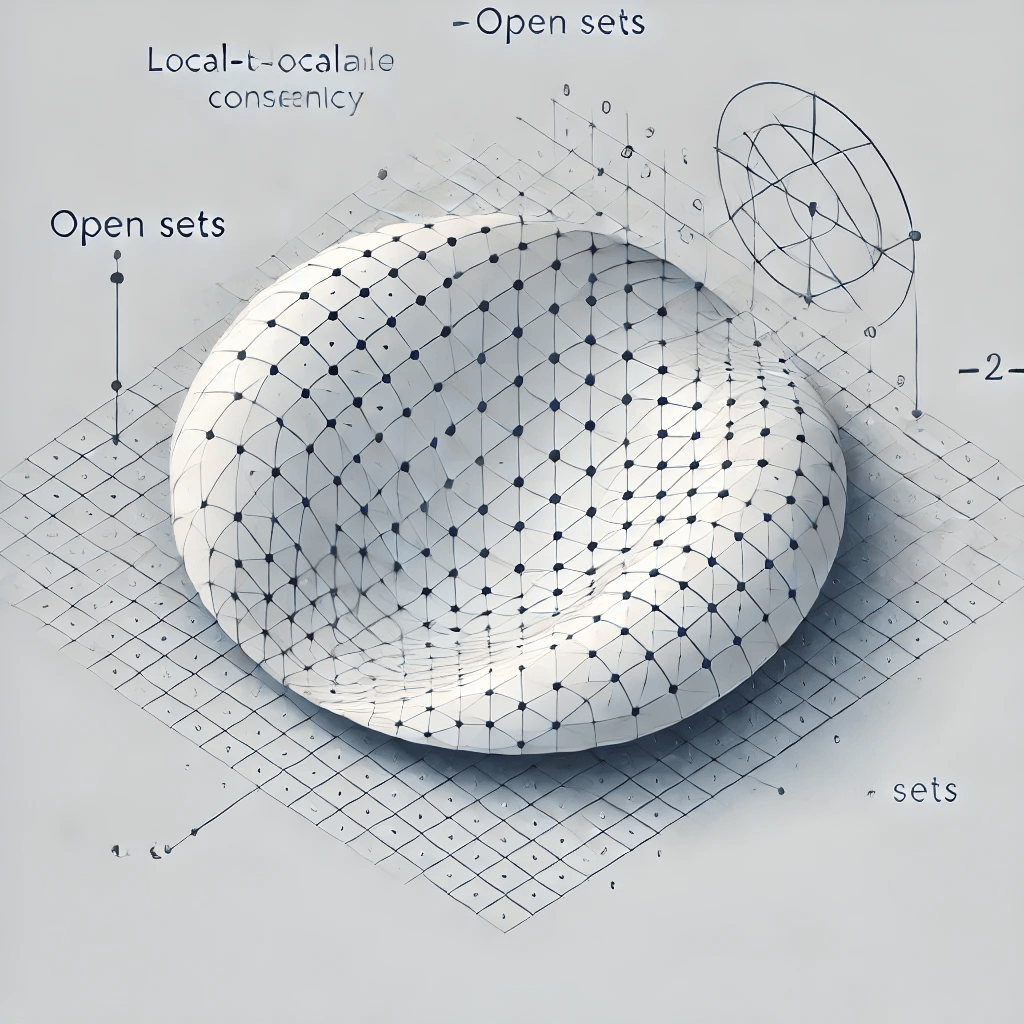
\includegraphics[width=0.8\textwidth]{sheaves.png}

    \caption{Sheaves help us define gluing conditions for consciousness (from local-to-global dynamics)}
\end{figure}

For any two overlapping regions $U$ and $V$, the sheaf includes restriction maps:

\begin{align}
\rho U \cap V: \mathcal{F}(U) \rightarrow \mathcal{F}(U \cap V)
\\
\rho V \cap U: \mathcal{F}(V) \rightarrow \mathcal{F}(U \cap V)
\end{align}


These maps must satisfy the crucial compatibility condition that for any sections $s \in \mathcal{F}(U)$ and $t \in \mathcal{F}(V)$:

$\rho U \cap V(s) = \rho V \cap U(t)$ on $U \cap V$

This compatibility ensures that local coherent states "glue" together properly across regional boundaries. The sheaf structure thus formalizes how consciousness maintains both local specialization and global integration through coherent gluing conditions. These conditions can be expressed through diagrams:

$\mathcal{F}(U) \rightarrow \mathcal{F}(U \cap V) \leftarrow \mathcal{F}(V)$

where the arrows represent restriction maps that must commute for consciousness to maintain coherence.

To capture the rich dynamics of conscious processing, we enhance the basic sheaf structure with additional mathematical machinery. Let $s \in \mathcal{F}(U)$ represent a local section corresponding to a coherent energy state in region U. The section s can be represented as a tuple:

$s = (E, \psi, \phi, \tau)$

where:

- $E$ represents the energy configuration

- $\psi$ captures the electromagnetic field state

- $\phi$ describes chemical gradients

- $\tau$ encodes the transcriptomic profile influencing local dynamics

The global behavior of consciousness emerges from coherent sheaf dynamics, where multiple local sections must satisfy compatibility conditions across overlapping regions. For regions $U$, $V$, $W$ with non-empty intersections, we require:

1. Binary Compatibility:
$\rho_{U \cap V}(s_U) = \rho_{V \cap U}(s_V) \text{ on } U \cap V$

2. Triple Overlap Condition:
$\rho_{U \cap V \cap W}(s_U) = \rho_{V \cap W \cap U}(s_V) = \rho_{W \cap U \cap V}(s_W) \text{ on } U \cap V \cap W$

These conditions ensure hierarchical coherence stability. The framework introduces a coherence measure $\mu$ that quantifies the degree of alignment between local sections:

$\mu(s_U, s_V) = \int_{U \cap V} \|\rho_{U \cap V}(s_U) - \rho_{V \cap U}(s_V)\|^2 \,d\nu$

where $d\nu$ represents an appropriate measure on the overlap region. Conscious processing requires that $\mu$ remains below certain thresholds determined by the brain's energetic constraints.

The global section of consciousness, $S \in \mathcal{F}(X)$, must satisfy not only local coherence conditions but also maintain stability under coherent deformation operators $D\lambda$:

$D\lambda(S)|_U = s_U + \delta\lambda(s_U)$

where $\delta\lambda$ represents small perturbations that model the continuous adaptation of conscious states. The existence of stable global sections requires that:

$\sup\{\mu(D\lambda(S)|_U, D\lambda(S)|_V)\} < \varepsilon$

for some small $\varepsilon > 0$ across all overlapping regions $U$, $V$ and allowable deformations $\lambda$.

This sheaf-theoretic framework naturally extends to incorporate the dynamics of energy flows through a coherent energy complex, leading us to consider the stress-energy tensor formalism in the next section.

For readers interested in deepening their understanding of sheaf theory and its applications to consciousness and computation, several key texts provide valuable foundations. The classic introduction \cite{MacLane1992} offers a comprehensive treatment of sheaves in both geometric and logical contexts, particularly useful for understanding the mathematical underpinnings of local-to-global transitions. For those seeking a more modern treatment, \cite{Kashiwara2005} presents advanced perspectives on categories and sheaves that illuminate the formal structures underlying coherent integration. The application of sheaf theory to concurrent and interactive systems, as detailed in \cite{Goguen1992}, provides crucial insights into how sheaf-theoretic approaches can model complex, distributed processes. Of particular relevance to consciousness studies is \cite{Rushworth2018}, which develops a categorical framework for consciousness using sheaf theory, demonstrating how these mathematical tools can bridge local neural dynamics and global conscious states. For those interested in the broader philosophical implications, \cite{Rosen1991} explores how sheaf-theoretic concepts illuminate fundamental questions about biological organization and cognition. These works collectively demonstrate how sheaf theory provides a rigorous mathematical framework for understanding the emergence of unified conscious experience from distributed neural processes.

\section{Stress-energy Tensor}

The stress-energy tensor $T\mu\nu$ describes the flow and distribution of energy-momentum within conscious systems. For our purposes, we decompose it into subsystem-specific components:

$T_{\mu\nu} = T_{\mu\nu}^{(EM)} + T_{\mu\nu}^{(chem)} + T_{\mu\nu}^{(mech)} + T_{\mu\nu}^{(int)}$

where the superscripts denote electromagnetic, chemical, mechanical, and interaction terms respectively. The Jacobian of this tensor, $\partial_\sigma T_{\mu\nu}$, captures how energy flows change across space and time:

$\partial_\sigma T_{\mu\nu} = \frac{\partial T_{\mu\nu}}{\partial x^\sigma}$

This framework allows us to track energy flow patterns essential for conscious processing while maintaining compatibility with the sheaf-theoretic structure previously described.

\subsection{Jacobian of the Stress-Energy Tensor}

The Jacobian of the stress-energy tensor provides a mathematical framework for tracking how conscious processing emerges from coordinated energy flows. For each point $x$ in the brain's neural architecture, we can express the full dynamics through:

$\partial_\sigma T_{\mu\nu}(x) = \begin{pmatrix} 
\frac{\partial T_{00}}{\partial t} & \frac{\partial T_{0i}}{\partial t} & \frac{\partial T_{0j}}{\partial t} \\[1em]
\frac{\partial T_{i0}}{\partial x^k} & \frac{\partial T_{ij}}{\partial x^k} & \frac{\partial T_{ij}}{\partial x^l}
\end{pmatrix}$

where each component describes specific aspects of conscious computation:

1. Energy Flow Components:

- $\frac{\partial T_{00}}{\partial t}$ tracks changes in local energy density

- $\frac{\partial T_{0i}}{\partial x^k}$ describes spatial energy flux gradients

- $\frac{\partial T_{0i}}{\partial x^k}$ captures stress propagation

2. Subsystem-Specific Terms:
For each subsystem $\alpha$ (electromagnetic, chemical, mechanical), we have:

$\partial_\sigma T_{\mu\nu}(\alpha) + \sum_\beta C_{\mu\nu}(\alpha,\beta) = J_{\mu\nu}(\alpha)$

\text{where:}
\begin{itemize}
\item $C_{\mu\nu}(\alpha,\beta)$ represents coupling terms between subsystems
\item $J_{\mu\nu}(\alpha)$ represents the source terms
\end{itemize}

3. Interface Terms:
The framework introduces boundary terms $B_{\mu\nu}$ that capture energy exchange at interfaces between regions:

$B_{\mu\nu}(x) = [T_{\mu\nu}(\alpha)]_{\partial\Omega}$

These interface terms are crucial for maintaining coherent conscious processing across regional boundaries.

\begin{figure}[h]
    \centering
    
\includegraphics[width=0.8\textwidth]{jacobian.png}

    \caption{The Jacobian of the stress-energy tensor specifies the necessary information to describe energy flows in the brain.}
\end{figure}

\subsection{Coupling-interface Terms}

The coupling and interface terms in the stress-energy framework capture how different subsystems interact to maintain conscious coherence. These terms are essential for understanding how local energy dynamics combine into global conscious states.

For any two subsystems $\alpha$ and $\beta$, the coupling terms $C_{\mu\nu}(\alpha,\beta)$ can be expanded as:

$C_{\mu\nu}(\alpha,\beta) = \gamma(\alpha,\beta)[\partial_\nu\phi(\alpha)\partial_\mu\phi(\beta) - \eta_{\mu\nu}(\partial_\lambda\phi(\alpha)\partial^\lambda\phi(\beta))]$

\text{where:}
\begin{itemize}
\item $\gamma(\alpha,\beta)$ represents coupling strength
\item $\phi(\alpha)$, $\phi(\beta)$ are field variables for each subsystem
\item $\eta_{\mu\nu}$ is the metric tensor
\item $\partial_\lambda$ denotes covariant derivatives
\end{itemize}

The interface terms at boundaries $\partial \Omega$ take the form:

$B_{\mu\nu}(x) = \sigma(x)[n \cdot \nabla T_{\mu\nu}] + \kappa(x)T_{\mu\nu}|_{\partial\Omega}$

\text{where:}
\begin{itemize}
\item $\sigma(x)$ represents interface conductivity
\item $n$ is the unit normal to the boundary
\item $\kappa(x)$ captures boundary resistance
\end{itemize}

These terms must satisfy conservation conditions:

$\int_{\partial\Omega} B_{\mu\nu}(x)\,dS + \int_\Omega C_{\mu\nu}(\alpha,\beta)\,dV = 0$

This ensures energy and information flow continuously across subsystem boundaries while maintaining coherent conscious states.

The total dynamics at interfaces must also satisfy coherent boundary conditions:

$\sum_{\alpha,\beta} [C_{\mu\nu}(\alpha,\beta) + \partial_\lambda B_{\mu\nu}(\alpha,\beta)] \leq \eta(x,t)$

where $\eta (x,t)$ represents the maximum allowable local deviation from perfect coherence, constrained by thermodynamic considerations. These conditions ensure that energy transfers between subsystems remain within bounds that support conscious processing.

The complete interface dynamics can be expressed through a hierarchy of coupling terms:

$C_{\mu\nu} = C^{(1)}_{\mu\nu} + C^{(2)}_{\mu\nu} + C^{(3)}_{\mu\nu} + \cdots$

where each order captures increasingly complex interactions between subsystems, with higher-order terms typically decreasing in magnitude:

$|C^{(n)}_{\mu\nu}| \sim O(\gamma^n)$

where $\gamma < 1$ is a coupling parameter.

The mathematical foundations of stress-energy tensors and their applications to complex dynamical systems can be further explored through several seminal works. A comprehensive introduction to the geometric foundations is presented in \cite{Frankel2011}, which provides essential background on tensor analysis and differential geometry. The classic treatment in \cite{Misner1973} offers deep insights into how stress-energy tensors describe the flow and distribution of energy-momentum in physical systems, while \cite{Landau1987} provides crucial perspectives on how these concepts apply to continuous media and field theories. For those interested in the quantum aspects of energy flow and coherence, \cite{Peskin1995} develops the mathematical framework necessary for understanding field-theoretic approaches to information integration. The relationship between stress-energy tensors and general covariance principles is thoroughly examined in \cite{Wald1984}, providing important context for understanding how local energy conservation emerges from global symmetries. These texts collectively establish the mathematical rigor needed to apply stress-energy tensor analysis to complex biological systems like the brain, where multiple forms of energy flow must maintain coherent relationships across various scales.

\section{Triangulation and Mutual Recursion}

The maintenance of conscious coherence requires not only proper coupling between subsystems but also continuous feedback and adjustment across regions. This leads us to incorporate triangulation and mutual recursion into our mathematical framework. Let R(x,t) represent the recursive operator that describes how local states update based on neighboring regions:

$R(x,t): T(x,t) \rightarrow T(x,t + \delta t)$

where triangulation ensures that for any three regions $A$, $B$, and $C$:

$\|R(A \rightarrow B) \circ R(B \rightarrow C) - R(A \rightarrow C)\| < \varepsilon$

This formalism captures how conscious states maintain consistency through continuous mutual adjustment.

The unity of consciousness across spatially separated regions presents a fundamental challenge that ECC addresses through coordinated triangulation and recursive updating. For non-adjacent regions A and C, separated by intermediate regions {Bi}, consciousness maintains coherence through recursive triangulation chains:

$R(A \rightarrow C) = \circ_{i} R(B_i \rightarrow B_{i+1})$

where the composition of local recursive operators must satisfy the global coherence condition:

$\|R(A \rightarrow C) - R(A \rightarrow B_1) \circ R(B_1 \rightarrow B_2) \circ \cdots \circ R(B_n \rightarrow C)\| < \varepsilon(d)$

Here, $\varepsilon(d)$ represents the maximum allowable deviation as a function of distance d between regions.

The triangulation operators $T(x,y,z)$ acting on any three regions must satisfy:

1. Consistency across paths:
$T(A,B,C) \approx T(A,B',C)$

for any alternative intermediate point $B'$, where $"\approx"$ indicates agreement within coherence bounds.

2. Mutual recursion stability:
$R^{(n+1)}(x) = F[R^{(n)}(y) \mid y \in N(x)]$

where:

- $R(n)$ represents the nth recursive update

- $N(x)$ is the neighborhood of point $x$

- $F$ is the recursive update function

This framework enables non-local coherence maintenance through:

$\|T(A,B,C) - T(A,B',C)\| \leq \kappa \exp(-\lambda d)$

where $\kappa$ and $\lambda$ are constants determining how quickly coherence can propagate across distance $d$.

This non-local coherence maintenance is further constrained by the recursive coherence bound:

$\sum_{x,y} \|R^{(n+1)}(x) - F[R^{(n)}(y)]\| \leq \eta(t)\exp(-\mu d(x,y))$

where $\eta(t)$ represents time-dependent coherence thresholds and $\mu$ describes the spatial decay of coherence. The total system must satisfy both local and global stability conditions:

$\text{Local: } \|R^{(n+1)}(x) - R^{(n)}(x)\| \rightarrow 0 \text{ as } n \rightarrow \infty$

$\text{Global: } \|T(A,B,C) - T(A',B',C')\| \leq \varepsilon \text{ for any valid triangulation triple}$

These mathematical structures provide the foundation for understanding how consciousness maintains unity across spatial and temporal separations, leading us to consider how these local mechanisms combine to create global conscious states in the next section.

Several foundational works provide deeper insight into the mathematical principles underlying triangulation and mutual recursion in complex systems. The seminal work \cite{Bird1988} establishes crucial foundations for understanding recursive patterns in functional systems, particularly relevant to how neural networks maintain stable recursive relationships. A rigorous treatment of fixed-point theory for recursive queries is presented in \cite{Alegre2017}, offering mathematical tools essential for analyzing how recursive processes achieve stable states in biological systems. For understanding the network theoretical aspects of triangulation, \cite{Erdos1959} provides fundamental insights into random graph theory that inform how triangulated relationships emerge and stabilize in neural networks. The biological implications of recursive organization are thoughtfully explored in \cite{Maturana1987}, which examines how living systems maintain coherence through recursive interactions. Building on this, \cite{Freeman2000} offers crucial perspectives on how mesoscopic brain dynamics emerge from recursive processes and triangulated relationships across neural populations. The relationship between recursion and consciousness is further illuminated in \cite{Hofstadter2007}, which explores how self-referential loops and recursive processes might contribute to conscious experience. These works collectively provide the theoretical foundation necessary for understanding how triangulation and mutual recursion contribute to the maintenance of conscious states through coherent energy dynamics.

\section{Local-to-Global Coherence}

The integration of sheaf theory, stress-energy tensors, and recursive triangulation provides a comprehensive mathematical framework for understanding how consciousness achieves coherent global states from local dynamics. Let $M$ represent the manifold of possible conscious states. The global section $S \in F(M)$ emerges from the interplay of local coherence mechanisms through the coherence integration equation:

$S = \int_M [T_{\mu\nu} \circ R \circ T](x) \,dV$

where the composition of stress-energy dynamics ($T\mu\nu$), recursive updates ($R$), and triangulation operators ($T$) must satisfy both local and global coherence conditions.

The global coherence of consciousness emerges from the satisfaction of multiple simultaneous constraints across all mathematical structures previously introduced:

1. Sheaf Coherence:
$\forall U,V \subseteq M: \rho_{U \cap V}(S|_U) = \rho_{V \cap U}(S|_V)$

2. Energy Conservation:
$\partial_\sigma T_{\mu\nu} + \sum_{\alpha,\beta} C_{\mu\nu}(\alpha,\beta) = 0$

3. Recursive Stability:
$\lim_{n \rightarrow \infty} \|R^{(n+1)} - R^{(n)}\| \rightarrow 0$

4. Triangulation Consistency:
$\sup_{A,B,C} \|T(A,B,C) - T(A',B,C)\| \leq \varepsilon$

These conditions must be simultaneously satisfied while maintaining thermodynamic efficiency:

$\eta = -\int_M T_{\mu\nu}\partial_\mu\xi_\nu \,dV \leq \eta_{\text{max}}$

where $\xi_\nu$ represents the Killing vector fields associated with energy conservation.

This mathematical framework, while abstract, finds direct physical implementation in biological neural systems. The translation from mathematical formalism to biological reality requires understanding how these structures are realized through specific biophysical mechanisms.

For deeper exploration of local-to-global coherence in neural systems, several foundational works provide crucial theoretical frameworks. The seminal work in \cite{Sporns2011} establishes fundamental principles for understanding how local neural dynamics integrate into global brain states through network organization. A rigorous treatment of coordination dynamics is presented in \cite{Bressler2016}, offering essential insights into how local neural populations achieve coherent relationships across multiple scales. The theoretical framework in \cite{Kelso2012} provides crucial perspectives on multistability and metastability in brain dynamics, particularly relevant to understanding how local coherence patterns contribute to global conscious states. Building on these foundations, \cite{Werner2013} examines consciousness through the lens of phase space dynamics and criticality, offering important insights into how local-to-global transitions emerge in neural systems. The relationship between electromagnetic field integration and consciousness is thoughtfully explored in \cite{McFadden2020}, which examines how local field potentials might contribute to global conscious integration. These perspectives are complemented by \cite{Tononi2015}, which provides a theoretical framework for understanding how information integration occurs across different scales in conscious systems. Collectively, these works establish the theoretical foundations necessary for understanding how local patterns of neural activity combine to create globally coherent conscious states through multiple mechanisms of integration and coordination.

Drawing from recent theoretical work in cognitive neuroscience and complex systems, coherence within Energetically Coherent Computing (ECC) represents a fundamental organizing principle that emerges from the coordinated interaction of multiple energy forms across neural systems. This coherence manifests through the synchronized integration of electromagnetic fields, ionic gradients, and metabolic processes that collectively give rise to conscious experience \cite{McFadden2020, Werner2013}.

The framework of coherence in ECC can be understood through several interconnected dimensions. At the physical level, coherence emerges from the synchronized alignment of energy flows across multiple spatial and temporal scales. This alignment enables large-scale integration while maintaining local specificity, creating conditions necessary for conscious processing \cite{Kelso2012}. The resulting patterns of energy organization demonstrate remarkable stability while preserving the flexibility required for adaptive response to changing conditions \cite{Freeman2007}.

From an informational perspective, coherence enables the integration of diverse neural processes into unified conscious states. This integration occurs through carefully orchestrated patterns of energy flow that maintain consistent relationships across sensory, cognitive, and motor systems \cite{Baars2007}. The resulting coherent states provide the foundation for the phenomenal unity of consciousness while enabling sophisticated information processing \cite{Tononi2015}.

The mathematical formalization of coherence through sheaf theory provides rigorous tools for understanding how local patterns of energy organization combine into global conscious states \cite{Rushworth2018}. This approach reveals how disruptions in coherence can lead to altered states of consciousness, whether through sleep, anesthesia, or pathological conditions. The sheaf-theoretic framework particularly illuminates how consciousness requires proper "gluing" of local coherent states across neural tissues \cite{Abramsky2008}.

Coherence in ECC also reflects fundamental principles of energetic efficiency, where neural systems achieve sophisticated information processing while minimizing unnecessary energy dissipation \cite{Dehaene2011}. This efficiency emerges through evolved patterns of organization that enable both stability and adaptability while respecting thermodynamic constraints \cite{Bressler2016}. The resulting balance between energy conservation and information processing capacity proves essential for maintaining conscious states.

The dynamic nature of coherent organization becomes particularly evident through coordination dynamics \cite{Kelso2012}. Rather than representing static patterns, coherence emerges from continuous processes of self-organization that maintain stability while enabling flexible response to changing conditions. This dynamic stability allows consciousness to persist through varying environmental demands while preserving essential organizational features \cite{Haken2012}.

Understanding coherence through ECC thus reveals fundamental principles about how consciousness emerges from physical processes while remaining grounded in rigorous mathematical formalism. This framework suggests new approaches to investigating consciousness while providing theoretical tools for understanding both normal function and pathological conditions \cite{Alexander2019}. The resulting synthesis bridges phenomenology and physics through careful attention to the organizing principles that enable conscious experience.

After establishing this mathematical framework for describing patterns of energetic coherence across multiple scales, we come to a fundamental insight: what emerges from these formalisms is not merely a description of energy dynamics, but a deep theory of computation itself. Computation lies at the heart of ECC - not as abstract symbol manipulation, but as physically embodied processes maintaining specific patterns of energetic coherence.

The mathematical tools developed above - from sheaf-theoretic models of local-to-global integration to the analysis of coherent energy flows through stress-energy tensors - reveal how biological systems achieve sophisticated information processing while remaining bound by physical constraints. This suggests a radical reconceptualization of computation itself, one that maintains rigorous connections to physical dynamics rather than abstracting away from them.

This naturally leads us to examine a fundamental question: What is computation? While traditional approaches treat computation as substrate-independent symbol manipulation, ECC suggests a different view - one where computation emerges from and remains inseparable from coherent physical processes. Understanding this distinction requires us to carefully examine our basic assumptions about the nature of computation itself in the next section.

\section{What is Computation?}

The classical theory of computation, developed through pioneering work on effective procedures and mechanical calculation, established computation as the manipulation of discrete symbols according to formal rules \cite{Turing1936}. However, ECC suggests that consciousness requires a fundamentally different kind of computation—one grounded in continuous, physically embodied energy flows rather than abstract symbol manipulation \cite{MacLennan2004}.

Traditional computational theory centers on the notion that any computation can be reduced to a sequence of simple, mechanical steps executed by an abstract machine \cite{Copeland2017}. The universal Turing machine demonstrated that all classical computation could be realized through the manipulation of discrete symbols on an infinite tape. The Church-Turing thesis suggested that any intuitively computable function could be computed by these equivalent formalisms, establishing a foundational principle for computer science \cite{Smith2002}.

However, these classical approaches share crucial assumptions that ECC challenges. First, they presume that information can be perfectly encoded in discrete states, while ECC argues that conscious processing requires continuous, analog-like states that cannot be \textbf{fully} captured by discrete representations \cite{vanGelder1995}. Second, the Church-Turing thesis implies that computation is independent of its physical implementation, whereas ECC contends that consciousness requires specific physical properties and energy dynamics that cannot be abstracted away \cite{Landauer1996}.

These theoretical tensions highlight fundamental questions about the nature of computation itself. While the Church-Turing thesis may capture the essence of abstract symbol manipulation, consciousness appears to require what \cite{Piccinini2015} terms natural computation—physically embodied processes that cannot be reduced to discrete symbolic operations. This suggests that understanding consciousness requires expanding our conception of computation beyond traditional algorithmic frameworks.

\begin{figure}[h]
    \centering
    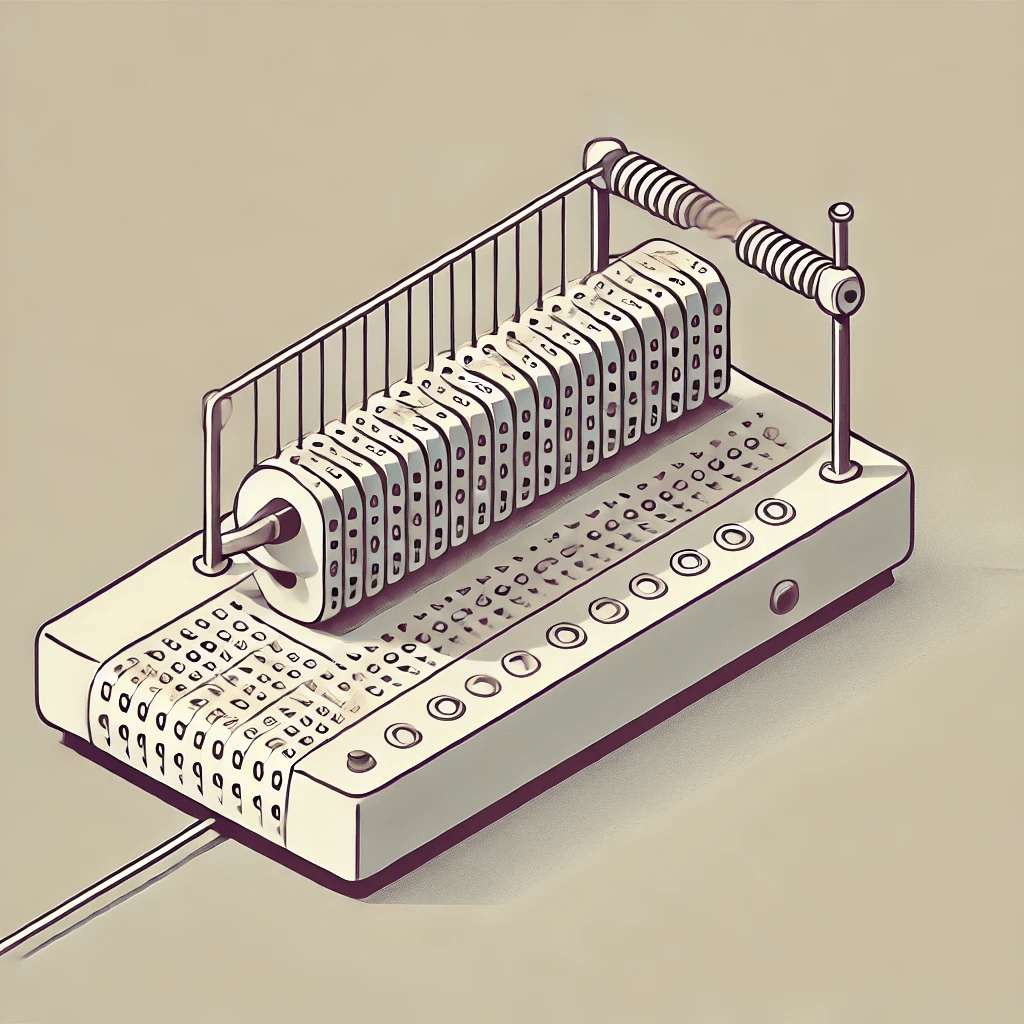
\includegraphics[width=0.8\textwidth]{turing.png}

    \caption{Artwork depicting a simple realization of an abstract Turing machine}
\end{figure}

The relationship between physical implementation and computation takes on particular significance in ECC's framework. While traditional computational theory treats physical substrates as incidental to computational processes \cite{Chalmers2011}, ECC suggests that certain physical properties—particularly those enabling coherent energy flows—are essential to conscious computation \cite{Landauer1996}. This perspective aligns with emerging understanding of how biological systems process information through continuous, physically grounded dynamics rather than discrete state transitions.

Recent theoretical work has begun to challenge the assumption that all natural processes admit computational description \cite{Searle1990}. Just as digestion cannot be adequately characterized as information processing, and gravitational phenomena cannot be reduced to computation, conscious experience may emerge from physical dynamics that resist computational abstraction \cite{vanGelder1995}. This aligns with growing skepticism about the computational theory of mind, particularly regarding the context-sensitivity and holistic nature of conscious thought.

TODO: G Ryle cite on category error below?

The framework suggests that attempting to reduce consciousness to computation represents what \cite{Smith2002} identifies as a category error—confusing the abstract map of computational description with the physical territory of conscious experience. While computational models may capture certain aspects of cognitive processing, they fundamentally miss the continuous, field-like properties that characterize conscious experience \cite{Piccinini2015}. This limitation becomes particularly evident when considering how consciousness maintains coherence across distributed neural processes.

Traditional computationalism faces particular challenges in explaining the temporal dynamics of consciousness \cite{Siegelmann2003}. The continuous flow of conscious experience appears fundamentally at odds with the discrete state transitions that characterize classical computation. ECC suggests that this temporal continuity emerges naturally from the physical dynamics of coherent energy flows, rather than requiring additional computational mechanisms to bridge discrete states.

The implications extend beyond theoretical understanding to practical questions about artificial consciousness \cite{Aaronson2013}. While digital computers excel at manipulating discrete symbols according to formal rules, they may be fundamentally incapable of supporting the specific forms of energetic coherence that ECC identifies as essential to conscious experience. This suggests that creating conscious artificial systems might require radically different approaches to computation and physical implementation.

The distinction between classical computation and conscious processing becomes particularly evident when examining how biological systems maintain coherent states across multiple scales \cite{MacLennan2004}. Unlike digital computers that maintain sharp boundaries between processing elements, conscious systems operate through continuous fields of influence that span multiple levels of organization. The resulting integration cannot be achieved through discrete computational steps but requires physical processes that maintain coherence through direct energetic interaction.

This perspective suggests a fundamental revision of how we understand computation in biological systems \cite{Adriaans2013}. Rather than viewing neural computation as analogous to digital processing, ECC proposes that conscious systems compute through patterns of energetic coherence that enable both stability and flexibility. This aligns with emerging views in theoretical neuroscience that emphasize the importance of continuous, dynamical processes in neural computation \cite{Piccinini2015}.

Recent work has begun to formalize these distinctions through mathematical frameworks that capture the continuous, field-like properties of conscious processing \cite{Siegelmann2003}. These approaches suggest that conscious computation operates in a fundamentally different regime from classical digital computation, one characterized by coherent energy flows rather than discrete state transitions. This mathematical perspective helps explain why consciousness exhibits properties that appear difficult or impossible to replicate through traditional computational approaches.

The relationship between energy and information takes on particular significance in this context \cite{Landauer1996}. While classical computation treats information as abstract and substrate-independent, ECC suggests that conscious processing requires specific physical implementations that enable particular patterns of energy flow and transformation. This perspective aligns with fundamental insights about the physical nature of information while suggesting new approaches to understanding how conscious systems process and integrate information.

The framework also provides insight into why certain aspects of conscious experience appear resistant to computational modeling \cite{Searle1990}. Features such as qualitative experience, temporal continuity, and global integration may emerge naturally from the physical dynamics of conscious systems while remaining fundamentally irreducible to discrete computational processes. This suggests that understanding consciousness requires moving beyond purely computational approaches to consider the physical basis of conscious experience.

This reconceptualization of computation through ECC's framework raises fundamental questions about the nature of conscious processing \cite{Wheeler1990}. While traditional approaches treat consciousness as emerging from abstract information processing, ECC suggests that conscious experience requires specific forms of physical organization that enable coherent energy dynamics. This perspective helps explain both the remarkable capabilities of conscious systems and their fundamental limitations.

The relationship between computation and physical implementation becomes particularly significant when considering the temporal aspects of conscious processing \cite{Deutsch2011}. Unlike classical computation, which proceeds through discrete time steps, consciousness exhibits continuous temporal evolution that emerges from the physical dynamics of neural systems. This temporal continuity appears essential to conscious experience yet proves difficult or impossible to capture through traditional computational frameworks.

Recent theoretical work has begun to explore how physical constraints shape the computational capabilities of conscious systems \cite{Fodor1981}. Rather than viewing these constraints as limitations to be overcome, ECC suggests they play a constructive role in enabling the specific forms of computation necessary for consciousness. This perspective aligns with emerging understanding of how biological systems achieve sophisticated information processing through their physical organization \cite{Smith2002}.

The framework provides particular insight into the relationship between local and global aspects of conscious computation \cite{vanGelder1995}. While traditional computational approaches often struggle to explain how distributed processing gives rise to unified experience, ECC suggests that this integration emerges naturally from the physical dynamics of coherent energy flows. This helps explain how consciousness achieves both differentiated processing and global coherence without requiring additional computational mechanisms.

These theoretical insights have important implications for understanding both biological consciousness and artificial systems \cite{Piccinini2015}. While digital computers may excel at certain forms of information processing, they appear fundamentally limited in their ability to support the specific types of computation that ECC identifies as essential to consciousness. This suggests that creating conscious artificial systems might require radically different approaches to computation and physical implementation.

The distinction between classical and conscious computation illuminates fundamental questions about the nature of mind and experience \cite{Chalmers2011}. ECC suggests that consciousness represents a unique form of physical computation that cannot be reduced to abstract symbol manipulation or discrete state transitions. This perspective helps resolve longstanding debates about the relationship between computation and consciousness while suggesting new directions for research and development.

The apparent tension between ECC's non-computational account of consciousness and its retention of "computation" in its name resolves through careful consideration of how the framework redefines computation itself \cite{MacLennan2004}. Rather than rejecting computation entirely, ECC reconceptualizes it as emerging from physical dynamics that maintain specific patterns of energetic coherence. This broadened understanding of computation aligns with recent theoretical work suggesting that biological systems compute through continuous, physically-grounded processes rather than discrete symbolic operations \cite{Siegelmann2003}. ECC accepts that consciousness implies computation but not vice versa.

This theoretical synthesis has important implications for both cognitive science and artificial intelligence \cite{Deutsch2011}. While traditional computational approaches have yielded significant insights into many aspects of cognition, consciousness appears to require forms of physical computation that go beyond classical frameworks. Understanding these distinctions may prove crucial for developing artificial systems that could potentially support conscious-like processing \cite{Aaronson2013}.

The framework thus suggests a fundamental revision in how we understand the relationship between computation and consciousness \cite{Wheeler1990}. Rather than treating consciousness as an emergent property of abstract computation, ECC positions it as arising from specific forms of physical computation that maintain coherent energy dynamics across multiple scales. This perspective provides new insights into both the possibilities and limitations of conscious systems while suggesting productive directions for future research and development \cite{Landauer1996}.

\newpage
\section{References}
\printbibliography[title={},heading=subbibliography]
%\printbibliography[title={References: Theoretical Framework}]
\end{refsection}